\section{Introduction}
\label{sec:intro}

Vision-language models (VLMs) have become the default tool for training-free visual anomaly detection (VAD): a practitioner uploads a query image, optionally attaches one or two normal reference images, and asks the model whether the query is abnormal. This recipe drives much of the recent published progress on industrial~\citep{gu2024anomalygpt,jeong2023winclip}, medical~\citep{bao2024bmad}, and cross-domain~\citep{jiang2024mmad} benchmarks. The appeal is obvious: no training, no architecture changes, and a single VLM call per image.

\begin{figure}[t]
    \centering
    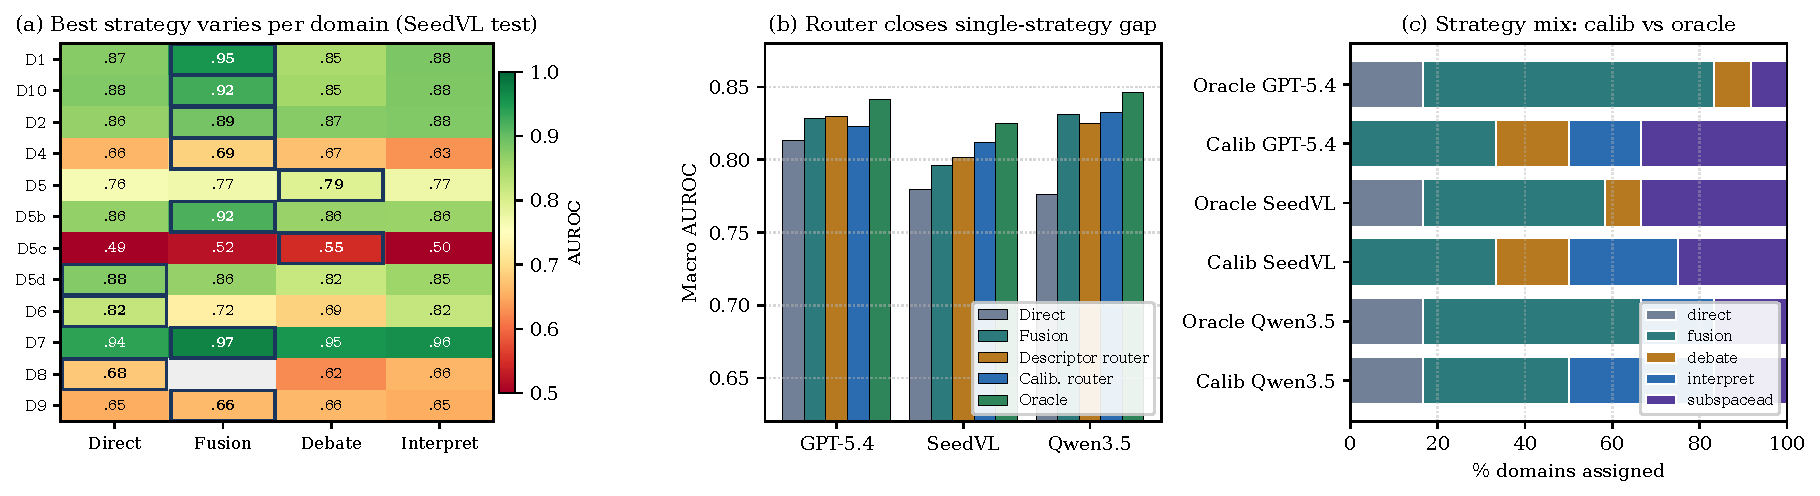
\includegraphics[width=\linewidth]{figures/fig_intuition.pdf}
    \caption{\textbf{AnomalyClaw on CrossDomainVAD-12 (design-motivation context, earlier evaluation split).}
    \textbf{(a)} No single strategy wins uniformly across domains: the best direct/fusion/debate/interpret cell differs by family (industrial, medical, logical, GI, change, road). \textbf{(b)} A calibration-driven router matches or beats the strongest single strategy on all three backbones and captures 40--60\% of the oracle gap; a zero-data descriptor router recovers much of the gain for free. \textbf{(c)} Per-domain strategy assignment is well-aligned with the oracle (9--10/12 agreement across backbones). This figure motivates AnomalyClaw's design (an always-on parallel-Direct branch alongside an autonomous refutation agent) by showing that no single strategy is uniformly best; final headline numbers are in Table~\ref{tab:main_results}, computed on the final CrossDomainVAD-12 test split.}
    \label{fig:intuition}
\end{figure}

Two observations drive this work. First, a cross-domain VAD deployment must handle textural industrial defects, semantic road obstacles, brain-MRI lesions, infrastructure cracks, and 3D industrial product renders with the same pipeline. The same fixed recipe---no matter how clever---cannot be optimal on all of them simultaneously: on our 12-domain test split, the argmax strategy varies by domain family and per-domain strategy selection is worth several pp of macro AUROC (Figure~\ref{fig:intuition}a). Second, recent ``agentic VAD'' systems~\citep{zhang2025agentiad,chen2026eagle,wei2025autoiad} bundle three decisions---what the VLM attends to, which expert provides evidence, and how to aggregate---into a single monolithic pipeline that is hard to ablate and hard to compare against simpler baselines; a related concern is that a stronger agent does not always beat a plain Direct VLM on every backbone, and a pipeline that \emph{only} reports the agent's final score silently loses when the agent is the weaker estimator.

We argue that these three decisions should be explicit and decoupled. We introduce \textbf{AnomalyClaw}, a training-free VAD agent organised around three orthogonal axes:

\begin{itemize}
    \item \textbf{Tools} --- zero-VLM-call primitives (domain descriptor, reference retriever, hotspot cropper, component counter, knowledge lookup).
    \item \textbf{Experts} --- frozen, pre-computed, non-parametric detectors (SubspaceAD~\citep{subspacead2026}, DINOv2 patch-$k$-NN, DINOv2 global).
    \item \textbf{Strategies} --- inference schemes that combine tools, experts, and VLM calls (direct, fusion, debate, interpret).
\end{itemize}

A lightweight \emph{router} selects a (tools, expert, strategy) triple per image. The router comes in two flavours: \emph{descriptor rules} (one rule per domain family, frozen once from the benchmark descriptor, no labelled data) and \emph{calibration argmax} (per-domain argmax over 20 labelled calibration items). An online expert-signal override can promote any domain to the \emph{interpret} strategy when patch-$k$-NN detects a spatially concentrated anomaly that the VLM missed.

\paragraph{Contributions.}
\begin{enumerate}
    \item \textbf{An always-on parallel-Direct branch inside an autonomous agent.} A single per-item invocation of AnomalyClaw runs a descriptor-free Direct VLM call and a multi-turn tool-using refutation trajectory in parallel on the same backbone, returning their fixed-weight average $s_{\mathrm{final}}{=}0.5\!\cdot\!s_{\mathrm{Direct}}+0.5\!\cdot\!s_{\mathrm{agent}}$. The ensemble is positive-in-mean on all three backbones and significant at $95\%$ on two: GPT-5.4 macro AUROC $0.731{\to}0.772$ ($+4.01$~pp, $P{=}1.000$), SeedVL $0.678{\to}0.738$ ($+5.99$~pp, $P{=}1.000$), Qwen3.5-VL-27B $0.714{\to}0.732$ ($+1.69$~pp, $P{=}0.971$ --- mean positive but $95\%$ CI $[-0.08,+3.51]$ touches zero).
    \item \textbf{Failure-mode robustness.} The agent is not individually better than Direct on every backbone: on Qwen3.5-VL-27B the agent alone is significantly \emph{worse} than Direct ($-4.46$~pp, $P{=}0.001$), yet the ensemble still improves over Direct. This robustness is the load-bearing property of the design and the reason the Direct branch is always-on rather than conditionally invoked. The agent and Direct make complementary per-domain errors on every backbone tested, including when the agent is the weaker estimator globally.
    \item \textbf{Task-anchored domain descriptors (context finding from earlier evaluation).} On an earlier design-exploration twelve-domain split, task-anchored descriptors uniformly beat generic ones on all three backbones at zero inference cost ($+6.4/+4.1/+3.2$ pp). Our main system intentionally runs its Direct branch in descriptor-\emph{free} mode to match the agent's task preamble; the descriptor finding motivates why adding domain-specific hints is valuable but is orthogonal to the ensemble claim.
    \item \textbf{Semi-supervised controller extension.} When $40$ dev labels per domain are available, we can add a learned Controller VLM on top of AnomalyClaw's two branches (\S\ref{sec:controller}). The Controller reads both branches' score--rationale pairs and a short retrieved rulebook; rules are built offline from disagreement-based routing meta-rules plus reused reference-only invariants and oracle corrective rules. On Qwen3.5-VL-27B the controller extension gives $0.7333{\to}0.7539$ ($+2.05$~pp, $P{=}0.995$) over the passive ensemble. A branch-frozen ablation with a wrong-domain negative control shows rule \emph{content} is the mechanism: empty and shuffled-rule controllers do not beat the passive ensemble, while correct rules do. The controller is a single-backbone case study on the weakest-ensemble backbone; we do not claim AnomalyClaw's training-free status extends to the controller extension.
    \item \textbf{Benchmark and framework release.} We release \textbf{CrossDomainVAD-12} (12 domain codes D1--D12, $1{,}418$ test items, calibration/dev/test splits), the full AnomalyClaw implementation (refutation agent with parallel Direct), the controller extension and offline rulebook-learning pipeline, the 13-tool library, the legacy Tool/Expert/Strategy registry and calibration-argmax router from the design-exploration phase, and stratified paired bootstrap confidence intervals for every headline comparison.
\end{enumerate}
